% Provenance (never printed): see sources/outline_sources.md (Year 2: radiogenic tracers
% Sr, Nd, Pb and mantle reservoirs; crustal growth; stable isotopes, delta notation and
% fractionation, d18O and d13C). Curves from figdata/bachelor-2/isotopes.py; exercise and
% problem values in the Book 4 scratch calculators calc/ch04.py and calc/ch04pb.py.
% Ruling (Sync 2): delta value and fractionation factor are chemistry's (Year 3 volume),
% recalled; this chapter defines the reference standards and the meteoric water line.
\chapter{Isotope Geochemistry}\label{ch:b2:isotope-geochemistry}

Mangaia, in the southern Pacific, and Tristan da Cunha, in the southern
Atlantic, are both volcanic islands built of basalt, and a hand specimen from
one looks much like a hand specimen from the other, or from a mid-ocean ridge.
Their isotopes tell them apart. The strontium of the Mangaia basalts carries
the same proportion of strontium-87 as that of the ridges, about
$^{87}\mathrm{Sr}/^{86}\mathrm{Sr} = 0.7028$, while their lead is among the most
radiogenic on Earth, with $^{206}\mathrm{Pb}/^{204}\mathrm{Pb}$ near 21.6 against
18.4 for the ridges. The Tristan basalts hold more strontium-87, 0.7050 to
0.7054, and less neodymium-143 than either. Melting does not sort isotopes of
these heavy elements, so each lava carries the isotopic signature of the
mantle that melted to make it: the Earth's mantle is not one reservoir but
several, which have kept different parent--daughter ratios for billions of
years. This chapter uses the radioactive decay of rubidium, samarium, uranium
and thorium as a set of tracers, follows the evolution of the mantle and the
continental crust through the neodymium isotopes, separates the mantle into
reservoirs and mixtures of reservoirs, discusses how fast the continents grew,
and ends with the light stable isotopes of oxygen, hydrogen and carbon, which
trace water and carbon through the Earth.
% ledger: data:b4-oib-isotopes, gale13:isotopes

\begin{recall}
A radioactive parent decays at the rate $\lambda P$, and in a closed system the
daughter ratio grows as $(D/D_s)_{\text{now}} = (D/D_s)_0 + (P/D_s)_{\text{now}}
(e^{\lambda t}-1)$, $D_s$ being a stable isotope of the daughter; minerals or
rocks formed together lie on an isochron, whose slope gives the age and whose
intercept gives the initial ratio (high-school volume, final year; Year 1 volume,
chapter on radiometric dating). A mass spectrometer separates ions by their
mass-to-charge ratio (chemistry books' Year 2 volume). The $\delta$ value of a
sample is $\delta = (R_{\text{sample}}/R_{\text{standard}} - 1)\times 1000$, in per
mil, and the fractionation factor between two phases A and B is
$\alpha_{\mathrm{A/B}} = R_{\mathrm A}/R_{\mathrm B}$, $R$ being the ratio of the
heavy to the light isotope; both are introduced, with the zero-point energies
that cause isotope fractionation, in the chemistry books' Year 3 volume.
\omterm{def:b2:elements-in-the-earth:partition}{Incompatible elements}, MORB and OIB were defined in
\cref{ch:b2:elements-in-the-earth}.
\end{recall}

\section{Radiogenic isotopes as tracers}

Three decay systems carry most of the information on the mantle and the crust.
Rubidium-87 decays to strontium-87, samarium-147 to neodymium-143, and uranium
and thorium, through their decay chains, to three isotopes of lead. Each parent
and daughter differ in their behaviour during melting, and each daughter has a
stable, non-radiogenic isotope against which it is measured.

\begin{table}[ht]
\centering
\begin{tabular}{lllll}
\hline
parent & daughter & ratio measured & decay constant (per year) & half-life (Ga)\\
\hline
$^{87}$Rb & $^{87}$Sr & $^{87}\mathrm{Sr}/^{86}\mathrm{Sr}$ & \num{1.3972e-11} & 49.6\\
$^{147}$Sm & $^{143}$Nd & $^{143}\mathrm{Nd}/^{144}\mathrm{Nd}$ & \num{6.524e-12} & 106.25\\
$^{238}$U & $^{206}$Pb & $^{206}\mathrm{Pb}/^{204}\mathrm{Pb}$ & \num{1.55125e-10} & 4.47\\
\hline
\end{tabular}
\caption{Three long-lived decay systems used as tracers. Data: IUPAC--IUGS
recommendations (Villa and others, 2020 and 2022).}
\label{tab:b2:isotope-geochemistry:decay}
\end{table}
% ledger: villa22:rb87, villa20:sm147

\begin{definition}[Radiogenic isotope tracer]\label{def:b2:isotope-geochemistry:tracer}
A \emph{radiogenic isotope tracer}\index{radiogenic isotope tracer} is the ratio
of a daughter isotope produced by a long-lived radioactive parent to a stable
isotope of the same element, such as $^{87}\mathrm{Sr}/^{86}\mathrm{Sr}$ or
$^{143}\mathrm{Nd}/^{144}\mathrm{Nd}$, used to identify the source of a rock rather
than to date it. The ratio of a reservoir grows at a rate set by its
parent--daughter ratio, and so records the history of that ratio.
\end{definition}

The two elements of a decay pair are separated whenever the mantle melts. In
\cref{ch:b2:elements-in-the-earth}, rubidium proved more incompatible than
strontium and neodymium more incompatible than samarium. A melt, and the crust
it builds, therefore leaves the mantle with a high Rb/Sr and a low Sm/Nd; the
residue keeps a low Rb/Sr and a high Sm/Nd. Over time the crust gains
strontium-87 faster than its source and neodymium-143 more slowly; the \omterm{def:b2:isotope-geochemistry:reservoirs}{depleted
mantle} does the opposite. The ratios of the two pairs move in opposite
directions, a point the Sr--Nd diagram below makes plain.

\begin{proposition}[Isotope ratios survive melting]\label{prop:b2:isotope-geochemistry:melting}
When a rock melts and the melt separates from the residue, the
$^{87}\mathrm{Sr}/^{86}\mathrm{Sr}$ and $^{143}\mathrm{Nd}/^{144}\mathrm{Nd}$ ratios of
the melt equal those of the source to within the precision of the
measurements; only the parent--daughter ratios, Rb/Sr and Sm/Nd, are changed.
\end{proposition}
\admitted

\noindent The statement rests on two facts. The isotopes of one element have the
same electronic structure, so they enter a crystal or a melt almost equally; the
relative mass difference between strontium-87 and strontium-86, about one per
cent, is far smaller than for oxygen or hydrogen, and at high temperature the
logarithm of an equilibrium fractionation factor falls as the inverse square of
the temperature, towards 1. And the measurement itself corrects the
fractionation that takes place in the mass spectrometer by fixing a ratio of two
non-radiogenic isotopes (for neodymium, $^{146}\mathrm{Nd}/^{144}\mathrm{Nd} =
0.7219$), which would erase any small natural fractionation as well. A lava,
therefore, samples the isotope ratios of its source, while its trace-element
ratios also reflect the melting.
% ledger: white:chur, white:t-dependence

\section{The evolution of mantle and crust}

\subsection{The chondritic reservoir}

Samarium and neodymium are both refractory lithophile rare earths
(\cref{ch:b2:elements-in-the-earth}): the \omterm{def:b2:elements-in-the-earth:bse}{bulk silicate Earth} should have kept
their chondritic ratio. The \omterm{def:b2:planet-formation-meteorites:chondrule}{chondrites} then give the Sm--Nd history of the
undifferentiated Earth.

\begin{definition}[Chondritic uniform reservoir]\label{def:b2:isotope-geochemistry:chur}
The \emph{chondritic uniform reservoir}\index{chondritic uniform reservoir}
(CHUR) is a model reservoir with the samarium--neodymium composition of the
\omterm{def:b2:planet-formation-meteorites:chondrule}{chondrites}, closed since the formation of the Solar System. Its present
ratios are $(^{143}\mathrm{Nd}/^{144}\mathrm{Nd})_{\mathrm{CHUR}} = 0.512638$ and
$(^{147}\mathrm{Sm}/^{144}\mathrm{Nd})_{\mathrm{CHUR}} = 0.1966$.
\end{definition}
% ledger: white:chur

Run backwards with the isochron equation, CHUR had, when the first solids
condensed \qty{4567}{Myr} ago (\cref{ch:b2:planet-formation-meteorites}),
\[
  ^{143}\mathrm{Nd}/^{144}\mathrm{Nd} = 0.512638 - 0.1966\,\bigl(e^{\lambda\cdot
  \num{4.567e9}\,\mathrm{yr}}-1\bigr) = 0.506692 .
\] Since then its ratio has grown by
1.2 per cent. The differences between terrestrial rocks are a thousand times
smaller, and are quoted in a more convenient unit.
% ledger: lugaro:cai, villa20:sm147

\begin{definition}[Epsilon notation]\label{def:b2:isotope-geochemistry:epsilon}
The \emph{epsilon notation}\index{epsilon notation} expresses the
$^{143}\mathrm{Nd}/^{144}\mathrm{Nd}$ ratio of a sample, at a time $t$ before the
present, as its relative deviation from CHUR at the same time, in parts per ten
thousand:
\[
  \varepsilon_{\mathrm{Nd}}(t) = \left(
  \frac{(^{143}\mathrm{Nd}/^{144}\mathrm{Nd})_{\text{sample}}(t)}
       {(^{143}\mathrm{Nd}/^{144}\mathrm{Nd})_{\mathrm{CHUR}}(t)} - 1\right)\times 10^4 .
\]
Without a time, $\varepsilon_{\mathrm{Nd}}$ is the present value.
\end{definition}

The mean MORB, with $^{143}\mathrm{Nd}/^{144}\mathrm{Nd} = 0.513074$, has
$\varepsilon_{\mathrm{Nd}} = (0.513074/0.512638 - 1)\times10^4 = +8.5$; most rocks
lie between $-20$ and $+10$. A positive value means that the source of the rock
has had, on average over the Earth's history, a higher Sm/Nd than the
\omterm{def:b2:planet-formation-meteorites:chondrule}{chondrites}: it is depleted in the more \omterm{def:b2:elements-in-the-earth:partition}{incompatible element}, neodymium. A
negative value means the opposite. The departure from the chondritic Sm/Nd is measured by the
fractional deviation
\[
  f_{\mathrm{Sm/Nd}} = \frac{(\mathrm{Sm}/\mathrm{Nd})_{\text{sample}}}
  {(\mathrm{Sm}/\mathrm{Nd})_{\mathrm{CHUR}}} - 1,
\]
which is the same whether the ratios are by mass or by atoms. With the CI values
of \cref{ch:b2:elements-in-the-earth} (Sm 0.145, Nd \qty{0.457}{ppm},
$\mathrm{Sm}/\mathrm{Nd} = 0.317$), the upper continental crust (4.7 and
\qty{27}{ppm}, 0.174) has $f_{\mathrm{Sm/Nd}} = -0.45$.
% ledger: gale13:isotopes, white:chur, lodders:ci-table, rg03:ucc-trace

\begin{proposition}[Linear growth of $\varepsilon_{\mathrm{Nd}}$]\label{prop:b2:isotope-geochemistry:linear}
A reservoir that separated from CHUR and has kept the fractional deviation
$f_{\mathrm{Sm/Nd}}$ since then changes its $\varepsilon_{\mathrm{Nd}}$, forward in
time, at the rate
\[
  \frac{\mathrm{d}\varepsilon_{\mathrm{Nd}}}{\mathrm{d}\tau} \approx Q\,f_{\mathrm{Sm/Nd}},
  \qquad
  Q = 10^4\,\lambda_{147}\,
  \frac{(^{147}\mathrm{Sm}/^{144}\mathrm{Nd})_{\mathrm{CHUR}}}
       {(^{143}\mathrm{Nd}/^{144}\mathrm{Nd})_{\mathrm{CHUR}}}
  = \qty{25.0}{\per\giga\year},
\]
where $\tau$ is time counted forwards. A reservoir with $\varepsilon_0$ at its
separation, a time $T$ ago, has today $\varepsilon_{\mathrm{Nd}} \approx \varepsilon_0
+ Q f_{\mathrm{Sm/Nd}} T$.
\end{proposition}

\begin{proof}
Write $R$ for $^{143}\mathrm{Nd}/^{144}\mathrm{Nd}$ and $p$ for
$^{147}\mathrm{Sm}/^{144}\mathrm{Nd}$. In a closed reservoir
$\mathrm{d}R/\mathrm{d}\tau = \lambda p\,e^{\lambda t}$, with $t$ the time before the
present; as $\lambda t \le 0.03$, the factor $e^{\lambda t}$ differs from 1 by at
most 3 per cent, and $\mathrm{d}R/\mathrm{d}\tau \approx \lambda p$. Then
$\mathrm{d}(R_s - R_c)/\mathrm{d}\tau \approx \lambda (p_s - p_c) = \lambda p_c
f_{\mathrm{Sm/Nd}}$, since $p_s/p_c - 1 = f_{\mathrm{Sm/Nd}}$. Dividing by $R_c$,
which changes by only 1.2 per cent over the age of the Earth, gives
$\mathrm{d}\varepsilon/\mathrm{d}\tau \approx 10^4\lambda p_c f/R_c$. With
$\lambda = \qty{6.524e-12}{\per\year}$, $p_c = 0.1966$ and $R_c = 0.512638$, $Q =
\num{2.502e-8}$ per year, \qty{25.0}{\per\giga\year}.
\end{proof}
% ledger: villa20:sm147, white:chur

A crust with the Sm/Nd of the upper crust ($f = -0.45$) therefore loses about
11 epsilon units per billion years relative to CHUR, while a mantle reservoir
needs only $f = +0.07$ to climb from 0 to the MORB value of $+8.5$ in
\qty{4.567}{Ga}. The figure below follows the exact equations for three
reservoirs: CHUR, a \omterm{def:b2:isotope-geochemistry:reservoirs}{depleted mantle} closed since the Earth formed with the Sm/Nd
that brings it to the MORB value today ($^{147}\mathrm{Sm}/^{144}\mathrm{Nd} =
0.211$), and a crust extracted from that mantle 2.7 billion years ago with the
upper crust's Sm/Nd ($0.108$). The crust started at $\varepsilon_{\mathrm{Nd}} =
+3.5$, the value of its source at the time, and now stands at $-27$.

\begin{definition}[Depleted mantle, enriched mantle]\label{def:b2:isotope-geochemistry:reservoirs}
A \emph{depleted mantle}\index{depleted mantle} is a part of the mantle that has
lost \omterm{def:b2:elements-in-the-earth:partition}{incompatible elements} to melts, so that its Sm/Nd is higher and its Rb/Sr
lower than chondritic; with time its $\varepsilon_{\mathrm{Nd}}$ becomes positive and
its $^{87}\mathrm{Sr}/^{86}\mathrm{Sr}$ low. An \emph{enriched
mantle}\index{enriched mantle} is a part of the mantle that has gained
\omterm{def:b2:elements-in-the-earth:partition}{incompatible elements}, for instance from recycled crust or from small melts,
with a negative $\varepsilon_{\mathrm{Nd}}$ or a high $^{87}\mathrm{Sr}/^{86}\mathrm{Sr}$.
\end{definition}

\begin{omfigure}
\centering
\begin{tikzpicture}
\begin{axis}[omrecord, width=0.82\linewidth, height=6.4cm,
  x dir=reverse, xmin=0, xmax=4.6, ymin=-30, ymax=12,
  xlabel={time before present (Ga)}, ylabel={$\varepsilon_{\mathrm{Nd}}(t)$},
  tick label style={font=\scriptsize}, label style={font=\small}]
\addplot[thick, black] table[x=t_Ga, y=eps] {figdata/out/bachelor-2-isotopes-chur.dat};
\addplot[very thick, blue!70!black] table[x=t_Ga, y=eps] {figdata/out/bachelor-2-isotopes-dm.dat};
\addplot[very thick, brown!70!black] table[x=t_Ga, y=eps] {figdata/out/bachelor-2-isotopes-crust.dat};
\addplot[densely dashed, gray] coordinates {(2.7,-30) (2.7,12)};
\node[font=\scriptsize, anchor=north] at (axis cs:3.6,-0.6) {CHUR};
\node[font=\scriptsize, blue!70!black, anchor=south east] at (axis cs:0.4,8.8) {depleted mantle, $+8.5$};
\node[font=\scriptsize, brown!70!black, anchor=north east] at (axis cs:0.3,-25.5) {crust, $-27$};
\node[font=\scriptsize, gray, anchor=north west, align=left] at (axis cs:2.65,-12) {crust extracted\\at \qty{2.7}{Ga}};
\end{axis}
\end{tikzpicture}
\par\smallskip{\small Neodymium isotope evolution, as $\varepsilon_{\mathrm{Nd}}$, of
the chondritic reservoir (zero by definition), of a \omterm{def:b2:isotope-geochemistry:reservoirs}{depleted mantle} closed since
\qty{4.567}{Ga} whose Sm/Nd brings it to the mean MORB today, and of a crust
extracted from it \qty{2.7}{Ga} ago with the Sm/Nd of the upper continental
crust. Each line is nearly straight, as the linear-growth proposition says. Data:
CHUR, White's text; mean MORB, Gale and others (2013); Sm/Nd of the crust,
Rudnick and Gao.}
\end{omfigure}
% ledger: white:chur, villa20:sm147, gale13:isotopes, rg03:ucc-trace, lodders:ci-table, lugaro:cai

\subsection{Two complementary reservoirs}

If the continental crust and the \omterm{def:b2:isotope-geochemistry:reservoirs}{depleted mantle} were made from one chondritic
reservoir, their neodymium must add back to the chondritic value. Neodymium is
the carrier: each reservoir counts in proportion to the neodymium it holds.

\begin{proposition}[Isotope mass balance]\label{prop:b2:isotope-geochemistry:mass-balance}
Let reservoirs $i$ of masses $M_i$ and neodymium concentrations $C_i$ come from
the division of one parent reservoir. Then, to a very good approximation,
\[
  \sum_i M_i C_i\, \varepsilon_i = \Bigl(\sum_i M_i C_i\Bigr) \varepsilon_{\text{parent}},
\]
both sides being evaluated at the same time, and the parent being followed as if
it had stayed whole.
\end{proposition}

\begin{proof}
The number of $^{143}\mathrm{Nd}$ atoms and the number of $^{144}\mathrm{Nd}$ atoms
are each conserved by the division, and each later grows (for
$^{143}\mathrm{Nd}$) or stays (for $^{144}\mathrm{Nd}$) in each reservoir exactly as
in the whole. Hence the $^{144}\mathrm{Nd}$-weighted mean of the ratios $R_i$ equals
the ratio of the parent, $R_p$. The share of $^{144}\mathrm{Nd}$ in neodymium varies
between reservoirs by much less than a part in a thousand, so weighting by
$M_iC_i$ is the same as weighting by $^{144}\mathrm{Nd}$. Finally $\varepsilon$ is a
linear function of $R$ at a given time, $\varepsilon = 10^4(R/R_c - 1)$, and a
weighted mean of linear functions is the linear function of the weighted mean.
\end{proof}

With the upper-crust value of \qty{27}{ppm} of neodymium taken for the whole
crust, a continental crust of \qty{7.2e9}{km^3} at \qty{2830}{kg/m^3}, that is
\qty{2.0e22}{kg} or 0.51 per cent of the mass of the silicate Earth, holds
$0.0051\times27/1.25 = 11$ per cent of the silicate Earth's neodymium (\omterm{def:b2:elements-in-the-earth:bse}{primitive
mantle}, \qty{1.25}{ppm}). If the crust has an average $\varepsilon_{\mathrm{Nd}}$ of
$-15$, a negative contribution of $0.11\times15 = 1.65$ units must be
balanced by the mantle: a reservoir at the MORB value of $+8.5$ would need to hold
about a fifth of the silicate Earth's neodymium (\cref{exo:b2:isotope-geochemistry:9}). This is one of the
arguments that the \omterm{def:b2:isotope-geochemistry:reservoirs}{depleted mantle} sampled by the ridges is not the whole
mantle.
% ledger: cogley84:continents, cm95:crust, ms95:pm-trace, rg03:ucc-trace, data:prem, earth:mass, gale13:isotopes

\section{The reservoirs of the mantle}

The isotopic ratios of oceanic basalts sample the mantle without passing through
the continental crust. Plotted against each other, they show both the
complementarity of crust and \omterm{def:b2:isotope-geochemistry:reservoirs}{depleted mantle} and the existence of other
reservoirs.

Strontium and neodymium isotopes are anticorrelated in most oceanic basalts: a
lava with a high $\varepsilon_{\mathrm{Nd}}$ has a low
$^{87}\mathrm{Sr}/^{86}\mathrm{Sr}$. This band is called the mantle array; it follows
from the opposite behaviour of the two pairs during melting (rubidium less
compatible than strontium, samarium more compatible than neodymium). The mean
MORB lies at its depleted end, with $^{87}\mathrm{Sr}/^{86}\mathrm{Sr} = 0.702819$ and
$\varepsilon_{\mathrm{Nd}} = +8.5$. \omterm{def:b2:elements-in-the-earth:morb-oib}{Ocean island basalts} spread from there towards
lower $\varepsilon_{\mathrm{Nd}}$ and higher $^{87}\mathrm{Sr}/^{86}\mathrm{Sr}$, but not
along a single line.
% ledger: white:dm, gale13:isotopes

\begin{definition}[Mantle end-member]\label{def:b2:isotope-geochemistry:end-members}
A \emph{mantle end-member}\index{mantle end-member} is one of the extreme
isotopic compositions from which the Sr, Nd and Pb isotope ratios of oceanic
basalts can be built by mixing. Four are commonly named: DMM, the depleted
MORB mantle (low $^{87}\mathrm{Sr}/^{86}\mathrm{Sr}$, high $\varepsilon_{\mathrm{Nd}}$);
HIMU, for a high $\mu = {}^{238}\mathrm{U}/^{204}\mathrm{Pb}$ in its source
(very radiogenic lead, $^{206}\mathrm{Pb}/^{204}\mathrm{Pb}$ above 20, with low
$^{87}\mathrm{Sr}/^{86}\mathrm{Sr}$); EM1, \omterm{def:b2:isotope-geochemistry:reservoirs}{enriched mantle} 1 (moderately high
$^{87}\mathrm{Sr}/^{86}\mathrm{Sr}$, negative $\varepsilon_{\mathrm{Nd}}$, unradiogenic
lead); and EM2, \omterm{def:b2:isotope-geochemistry:reservoirs}{enriched mantle} 2 (high $^{87}\mathrm{Sr}/^{86}\mathrm{Sr}$).
\end{definition}
% ledger: white:end-members

\begin{omfigure}
\centering
\begin{tikzpicture}
\begin{axis}[omrecord, width=0.82\linewidth, height=6.6cm,
  xmin=0.7020, xmax=0.7064, ymin=-6, ymax=11,
  xlabel={$^{87}\mathrm{Sr}/^{86}\mathrm{Sr}$}, ylabel={$\varepsilon_{\mathrm{Nd}}$},
  xticklabel style={/pgf/number format/fixed, /pgf/number format/precision=4},
  scaled x ticks=false, legend pos=south west, legend cell align=left,
  legend style={font=\scriptsize}, tick label style={font=\scriptsize},
  label style={font=\small}]
\addplot[only marks, mark=*, mark size=1.3pt, red!70!black] table[x=sr, y=eps] {figdata/out/bachelor-2-isotopes-himu.dat};
\addlegendentry{HIMU type: St.\ Helena, Mangaia, Tubuai}
\addplot[only marks, mark=square*, mark size=1.2pt, brown!70!black] table[x=sr, y=eps] {figdata/out/bachelor-2-isotopes-em1.dat};
\addlegendentry{EM1 type: Tristan da Cunha, Gough}
\addplot[only marks, mark=diamond*, mark size=3pt, blue!70!black] table[x=sr, y=eps] {figdata/out/bachelor-2-isotopes-morb.dat};
\addlegendentry{mean MORB}
\addplot[densely dashed, gray] coordinates {(0.7020,0) (0.7064,0)};
\node[font=\scriptsize, gray, anchor=south east] at (axis cs:0.7063,0.1) {CHUR};
\draw[->, gray] (axis cs:0.7030,9.5) -- (axis cs:0.7046,0.8);
\node[font=\scriptsize, gray, anchor=west, align=left] at (axis cs:0.7036,6.5) {the mantle array:\\depleted to enriched};
\end{axis}
\end{tikzpicture}
\par\smallskip{\small Strontium and neodymium isotopes of 89 basalts from five
ocean islands and of the mean \omterm{def:b2:elements-in-the-earth:morb-oib}{mid-ocean ridge basalt}. The HIMU-type islands plot
below the main array, with the low strontium ratio of MORB but a lower
$\varepsilon_{\mathrm{Nd}}$; the EM1-type islands lie on the enriched side of CHUR.
Samoan lavas of the EM2 type reach $^{87}\mathrm{Sr}/^{86}\mathrm{Sr} = 0.7205$, far
off this scale to the right. Data: Stracke and others (2022), CC BY 4.0; Gale and
others (2013); Edwards and others (2019).}
\end{omfigure}
% ledger: data:b4-oib-isotopes, gale13:isotopes, edwards19:samoa, white:chur

The island groups of the figure above are not random. The St.~Helena group,
which includes the Austral Islands (Mangaia and Tubuai among them) and
Ascension, plots below the main array and has the most radiogenic lead
($^{206}\mathrm{Pb}/^{204}\mathrm{Pb}$ above 20; Mangaia reaches 21.5 to 22.0). The
Kerguelen group, Tristan da Cunha, Gough and Kerguelen, lies at moderately high
$^{87}\mathrm{Sr}/^{86}\mathrm{Sr}$ and negative $\varepsilon_{\mathrm{Nd}}$, always with
unradiogenic lead. The Society group, with Samoa and the Marquesas, defines a
shallower Sr--Nd trend reaching very high strontium ratios: two Samoan lavas
have $^{87}\mathrm{Sr}/^{86}\mathrm{Sr}$ of 0.7186 and 0.7205, higher than modern
seawater (0.7092). The St.~Helena, Kerguelen and Society groups are the HIMU,
EM1 and EM2 types.
% ledger: white:end-members, data:b4-oib-isotopes, edwards19:samoa

A ratio that differs between two parts of the mantle must have been
maintained by a difference in parent--daughter ratio for a long time: a
difference of 10 units of $\varepsilon_{\mathrm{Nd}}$ takes, by the linear-growth
proposition, 1 billion years at $f = 0.4$ or 4 billion years at $f = 0.1$. The
mantle reservoirs are therefore old. What they are is read from the
parent--daughter ratios their isotopes demand. HIMU needs a high U/Pb and a low
Rb/Sr over a long time, which fits oceanic crust that lost lead and rubidium
in the fluids released above a subduction zone and was then stored in the mantle
for one or two billion years. EM1 and EM2 need a low Sm/Nd and, for EM2, a high
Rb/Sr: the signature of material derived from the continents, such as recycled
sediment, or of mantle enriched by small melts. These interpretations are
debated; the measurements are not.
% ledger: white:end-members

\begin{omfigure}
\centering
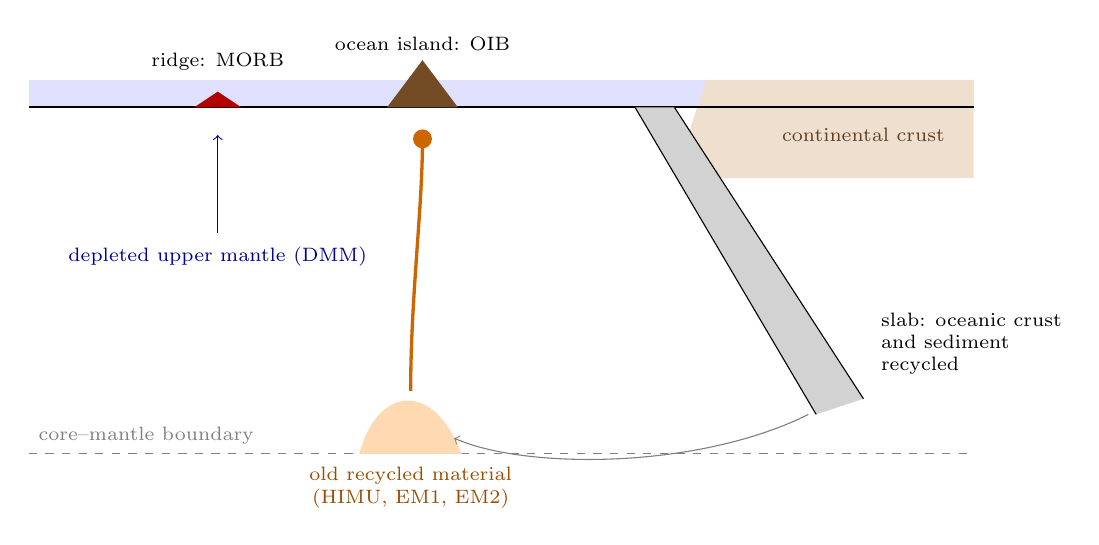
\begin{tikzpicture}[x=1cm, y=1cm, font=\scriptsize]
  % surface and lithosphere
  \fill[blue!12] (-6,0) rectangle (6,0.35);
  \fill[brown!25] (2.6,0.35) -- (6,0.35) -- (6,-0.9) -- (2.2,-0.9) -- cycle;
  \node[brown!50!black] at (4.6,-0.35) {continental crust};
  \draw[thick] (-6,0) -- (6,0);
  % ridge
  \node[anchor=south] at (-3.6,0.35) {ridge: MORB};
  \draw[->, blue!60!black] (-3.6,-1.6) -- (-3.6,-0.35);
  \node[blue!60!black, anchor=north] at (-3.6,-1.65) {depleted upper mantle (DMM)};
  % slab
  \fill[gray!35] (1.7,0) -- (2.2,0) -- (4.6,-3.7) -- (4.0,-3.9) -- cycle;
  \draw (1.7,0) -- (4.0,-3.9) (2.2,0) -- (4.6,-3.7);
  \node[anchor=west, align=left] at (4.7,-3.0) {slab: oceanic crust\\and sediment\\recycled};
  % deep pool and plume
  \draw[gray, dashed] (-6,-4.4) -- (6,-4.4);
  \node[anchor=south west, gray] at (-6,-4.4) {core--mantle boundary};
  \fill[orange!30] (-1.8,-4.4) .. controls (-1.6,-3.6) and (-0.9,-3.4) .. (-0.5,-4.4) -- cycle;
  \draw[very thick, orange!80!black] (-1.15,-3.6) .. controls (-1.15,-2.4) and (-1.0,-1.3) .. (-1.0,-0.4);
  \fill[orange!80!black] (-1.0,-0.4) circle (0.12);
  \fill[brown!60!black] (-1.45,0) -- (-1.0,0.6) -- (-0.55,0) -- cycle;
  \node[anchor=south] at (-1.0,0.6) {ocean island: OIB};
  \fill[red!70!black] (-3.9,0) -- (-3.6,0.2) -- (-3.3,0) -- cycle;
  \node[orange!60!black, anchor=north, align=center] at (-1.15,-4.45) {old recycled material\\(HIMU, EM1, EM2)};
  \draw[->, gray] (3.9,-3.9) .. controls (2.5,-4.6) and (0.3,-4.6) .. (-0.6,-4.2);
\end{tikzpicture}
\par\smallskip{\small One widely used interpretation of the mantle reservoirs, not to
scale: the ridges sample the depleted upper mantle; oceanic crust and sediment
return to the mantle at subduction zones; plumes rising from the deep mantle
bring up material in which old recycled components are mixed, and give the
islands their HIMU, EM1 or EM2 character.}
\end{omfigure}

\section{Mixing}

Many isotope arrays are mixtures. A lava may come from a source that is a
mixture of two reservoirs, or a magma may take in some of the crust it crosses.
The two cases obey the same algebra.

\begin{proposition}[Mixing hyperbola]\label{prop:b2:isotope-geochemistry:mixing}
Let a mixture contain a mass fraction $f$ of component A and $1-f$ of component
B. For an element of concentrations $C_{\mathrm A}$, $C_{\mathrm B}$ and isotope
ratios $R_{\mathrm A}$, $R_{\mathrm B}$:
\begin{enumerate}
\item the concentration of the mixture, $C = fC_{\mathrm A} + (1-f)C_{\mathrm B}$, and
its isotope ratio,
$R = \bigl(fC_{\mathrm A}R_{\mathrm A} + (1-f)C_{\mathrm B}R_{\mathrm B}\bigr)/C$, satisfy
$R = a + b/C$ with constants $a$ and $b$: the mixtures lie on a straight line in
a plot of $R$ against $1/C$;
\item two such ratios of two elements, $R$ and $R'$, lie on a hyperbola, called
the \emph{mixing hyperbola}\index{mixing hyperbola}, which is a straight line only
if the ratio of the two elements is the same in A and B. Its curvature is set by
$K = (C'/C)_{\mathrm A}/(C'/C)_{\mathrm B}$.
\end{enumerate}
\end{proposition}

\begin{proof}
(1) Eliminate $f$: $f = (C - C_{\mathrm B})/(C_{\mathrm A} - C_{\mathrm B})$. Then
$RC = C_{\mathrm B}R_{\mathrm B} + f(C_{\mathrm A}R_{\mathrm A} - C_{\mathrm B}R_{\mathrm
B})$ is linear in $C$, $RC = \alpha + \beta C$, and $R = \beta + \alpha/C$.
(2) The share of the element that comes from A is $s = fC_{\mathrm A}/C$, and $R =
R_{\mathrm B} + s(R_{\mathrm A} - R_{\mathrm B})$ is linear in $s$; likewise $R'$ is
linear in $s' = fC'_{\mathrm A}/C'$. With $u = f/(1-f)$, $s = u C_{\mathrm
A}/(uC_{\mathrm A} + C_{\mathrm B})$ and $s' = uC'_{\mathrm A}/(uC'_{\mathrm A} +
C'_{\mathrm B})$. Eliminating $u$ gives $s' = Ks/(1 + (K-1)s)$, a hyperbola in the
$(s, s')$ plane, hence in the $(R, R')$ plane; it is the straight line $s' = s$
when $K = 1$.
\end{proof}

\begin{omfigure}
\centering
\begin{tikzpicture}
\begin{axis}[omrecord, width=0.62\linewidth, height=6.2cm,
  xmin=0, xmax=1, ymin=0, ymax=1,
  xlabel={first ratio, rescaled (B $=0$, A $=1$)},
  ylabel={second ratio, rescaled},
  tick label style={font=\scriptsize}, label style={font=\small}]
\addplot[thick, red!70!black] table[x=x, y=y] {figdata/out/bachelor-2-isotopes-mixK50.dat};
\addplot[thick, black] table[x=x, y=y] {figdata/out/bachelor-2-isotopes-mixK10.dat};
\addplot[thick, blue!70!black] table[x=x, y=y] {figdata/out/bachelor-2-isotopes-mixK02.dat};
\node[font=\scriptsize, red!70!black, anchor=south east] at (axis cs:0.30,0.72) {$K=5$};
\node[font=\scriptsize, anchor=south east] at (axis cs:0.55,0.56) {$K=1$};
\node[font=\scriptsize, blue!70!black, anchor=north west] at (axis cs:0.62,0.22) {$K=0.2$};
\node[font=\scriptsize, anchor=north west] at (axis cs:0.0,0.0) {B};
\node[font=\scriptsize, anchor=south east] at (axis cs:1.0,1.0) {A};
\end{axis}
\end{tikzpicture}
\par\smallskip{\small Mixing curves between two components A and B for three
values of $K$, the ratio of the two elements in A divided by that in B. Each
isotope ratio is rescaled to 0 at B and 1 at A; the second element is $K$ times
richer in A, relative to the first, than in B, so the second ratio moves towards
A faster when $K > 1$.}
\end{omfigure}

A component rich in an element dominates the isotope ratio of that element in
the mixture. A recycled sediment holds tens of times more neodymium than the
\omterm{def:b2:isotope-geochemistry:reservoirs}{depleted mantle}, and a few per cent of it in a mantle source pulls the
$\varepsilon_{\mathrm{Nd}}$ of the mixture most of the way towards its own (problem).
The HIMU-type islands of the Sr--Nd figure lie off any mixing curve between MORB
and the EM1 islands: no mixture of two components explains all oceanic basalts,
and the end-members are at least four. A magma that assimilates continental
crust moves along a mixing curve towards the crust; its position on the curve
gives the proportion of crust taken in, a calculation taken up with crystallisation
in \cref{ch:b2:magmatic-differentiation}.

\section{Growth of the continental crust}

The continental crust is the complement of the \omterm{def:b2:isotope-geochemistry:reservoirs}{depleted mantle}; how fast it was
extracted is one of the oldest questions of isotope geochemistry, and still
open. Several records bear on it.

\begin{definition}[Crustal growth curve]\label{def:b2:isotope-geochemistry:growth}
A \emph{crustal growth curve}\index{crustal growth curve} gives the volume, or
mass, of continental crust in existence as a function of time, as a fraction of
the present volume. It reflects the balance between the generation of new crust
from the mantle and its destruction by recycling into the mantle.
\end{definition}

The rocks preserved today give a first curve: less than a quarter of the volume
of the juvenile continental crust preserved today is older than \qty{3}{Ga}, and
no known rock has a crystallisation age older than \qty{4.02}{Ga}. But the
preserved crust is what survived, not what was made. Other curves are built from
the neodymium isotopes of shales, which average the upper crust exposed to
erosion at the time they were deposited; from the hafnium isotopes of zircon
grains, which record whether the magma that crystallised them came from new or
reworked crust; or from the argon isotopes of hydrothermal quartz, which track
the degassing of the crust. Several recent models of this kind put at least 60
to 80 per cent of the present volume of continental crust in place by
\qty{3}{Ga}. The two views can be reconciled only if a great deal of early crust
was destroyed: in one box model fitted to both records, 2.3 to 2.6 times the
present volume of continental crust has been generated since the Earth formed,
and 1.3 to 1.6 times that volume has been returned to the mantle.
% ledger: dhuime18:growth

Present-day subduction zones show the recycling at work. Arc magmatism adds
about 2.5 cubic kilometres of new crust a year, 1.5 at intra-oceanic arcs and
1.0 at continental margins (2.7 as a long-term mean), while subduction carries
back about 3.2 cubic kilometres a year; to within the uncertainties, the
continents have not grown during at least the Phanerozoic. The isotopes of the \omterm{def:b2:isotope-geochemistry:end-members}{mantle
end-members}, which call for recycled crust and sediment, are the other side of
the same account.
% ledger: sv09:growth

\section{Stable isotopes}

The isotopes of the light elements, hydrogen, carbon, nitrogen, oxygen and
sulfur, are not produced by decay in measurable amounts. They are fractionated
instead by physical, chemical and biological processes, with relative mass
differences of up to a factor of two for hydrogen and deuterium, and their
variations are reported as $\delta$ values relative to agreed standards.

\begin{definition}[Isotope reference standard]\label{def:b2:isotope-geochemistry:standards}
An \emph{isotope reference standard}\index{isotope reference standard} is a
material whose isotope ratio defines the zero of a $\delta$ scale. Two are used
in the Earth sciences. \emph{VSMOW}\index{VSMOW} (Vienna Standard Mean Ocean
Water) defines $\delta\mathrm{D}$ and $\delta^{18}\mathrm{O}$ of waters, silicates and
most other materials; its absolute ratios are $\mathrm{D}/\mathrm{H} =
\num{1.5575e-4}$ and $^{18}\mathrm{O}/^{16}\mathrm{O} = \num{2.0052e-3}$.
\emph{VPDB}\index{VPDB} (Vienna Pee Dee Belemnite) defines $\delta^{13}\mathrm{C}$
and the $\delta^{18}\mathrm{O}$ of low-temperature carbonates; its absolute ratios
are $^{13}\mathrm{C}/^{12}\mathrm{C} = \num{1.1237e-2}$ and
$^{18}\mathrm{O}/^{16}\mathrm{O} = \num{2.0672e-3}$.
\end{definition}
% ledger: kc98:standards

The names recall the history: SMOW was an average ocean water, and PDB the
carbonate of a belemnite fossil from the Pee Dee formation; the original
materials ran out and were replaced by reference materials calibrated to them,
distributed by the International Atomic Energy Agency in Vienna and by NIST.
On the \omterm{def:b2:isotope-geochemistry:standards}{VSMOW} scale, the oxygen of \omterm{def:b2:isotope-geochemistry:standards}{VPDB} has $\delta^{18}\mathrm{O} = +30.9$ per mil
(\cref{exo:b2:isotope-geochemistry:2}): a marine carbonate is that much heavier than the ocean water it grew
from.
% ledger: kc98:standards

\subsection{Water}

Ocean water lies near $\delta^{18}\mathrm{O} = \delta\mathrm{D} = 0$, by the
definition of \omterm{def:b2:isotope-geochemistry:standards}{VSMOW}. Evaporation favours the light isotopes: at equilibrium
with liquid water at \qty{20}{\degreeCelsius}, with fractionation factors of
1.0098 for oxygen-18 and 1.084 for deuterium, the vapour would have
$\delta^{18}\mathrm{O} = 1000/1.0098 - 1000 = -9.7$ per mil and $\delta\mathrm{D} =
-77$ per mil; the vapour above the oceans is lighter still, about $-13$ per mil
in $\delta^{18}\mathrm{O}$, because evaporation is also a kinetic process.
As an air mass moves inland and towards the poles and cools, it rains out, and
each rain takes the heavy isotopes first; the remaining vapour, and the rain and
snow that follow, become lighter and lighter. Greenland ice typically has
$\delta^{18}\mathrm{O}$ of $-30$ to $-35$ per mil, Antarctic ice as low as $-50$.
% ledger: kc98:alpha, white:d18o

\begin{proposition}[Meteoric water line]\label{prop:b2:isotope-geochemistry:mwl}
Rain and snow from all over the world, and the fresh waters derived from them,
lie close to the \emph{meteoric water line}\index{meteoric water line}
\[
  \delta\mathrm{D} = 8\,\delta^{18}\mathrm{O} + 10 \quad\text{(per mil, VSMOW)},
\]
established empirically by Craig in 1961. Its intercept, 10 per mil, is called
the deuterium excess; individual regions have values between about 0 and 20.
\end{proposition}
\admitted

\noindent The slope can be understood without the full theory of condensation,
which is left to the Year 3 volume. In each step of condensation, the liquid
and the vapour differ by about $1000(\alpha - 1)$ per mil in each isotope, and
the two shifts stand in the ratio $(\alpha_{\mathrm D}-1)/(\alpha_{18}-1)$, which
is 8.6 at \qty{20}{\degreeCelsius} and 9.5 at \qty{0}{\degreeCelsius}: as the
vapour is depleted step by step, $\delta\mathrm{D}$ falls about eight times faster
than $\delta^{18}\mathrm{O}$. The intercept is not zero because the vapour leaving
the ocean is formed out of equilibrium. Ocean water, at the origin, therefore lies
below the line.
% ledger: kc98:mwl, kc98:alpha

\begin{omfigure}
\centering
\begin{tikzpicture}
\begin{axis}[omrecord, width=0.74\linewidth, height=6.4cm,
  xmin=-55, xmax=5, ymin=-440, ymax=60,
  xlabel={$\delta^{18}\mathrm{O}$ (per mil, VSMOW)}, ylabel={$\delta\mathrm{D}$ (per mil, VSMOW)},
  tick label style={font=\scriptsize}, label style={font=\small}]
\addplot[line width=4pt, gray!45] coordinates {(-35,-270) (-30,-230)};
\addplot[line width=4pt, gray!45] coordinates {(-50,-390) (-48,-374)};
\addplot[thick, blue!70!black] table[x=d18O, y=dD] {figdata/out/bachelor-2-isotopes-mwl.dat};
\addplot[only marks, mark=*, mark size=2pt, black] coordinates {(0,0)};
\node[font=\scriptsize, anchor=north west] at (axis cs:-3,-8) {VSMOW};
\addplot[only marks, mark=triangle*, mark size=2.4pt, red!70!black] coordinates {(-9.70,-77.5) (-11.56,-99.9)};
\node[font=\scriptsize, red!70!black, anchor=north, align=center] at (axis cs:-7,-118) {equilibrium\\vapour, 20\\and \qty{0}{\degreeCelsius}};
\node[font=\scriptsize, gray!50!black, anchor=north west] at (axis cs:-30,-240) {Greenland ice};
\node[font=\scriptsize, gray!50!black, anchor=west] at (axis cs:-47,-400) {Antarctic ice};
\draw[->, thick, gray] (axis cs:-6,-25) -- (axis cs:-24,-169);
\node[font=\scriptsize, gray!50!black, anchor=south east, align=right] at (axis cs:-12,-60) {colder: higher latitude,\\altitude, further inland};
\node[font=\scriptsize, blue!70!black, anchor=south east] at (axis cs:-36,-266) {$\delta\mathrm{D} = 8\,\delta^{18}\mathrm{O} + 10$};
\end{axis}
\end{tikzpicture}
\par\smallskip{\small The \omterm{prop:b2:isotope-geochemistry:mwl}{meteoric water line}. Precipitation becomes lighter as the
air that delivers it cools and rains out on its way to high latitudes, high
altitudes and continental interiors. Ocean water (\omterm{def:b2:isotope-geochemistry:standards}{VSMOW}) lies below the line;
the vapour in equilibrium with it, computed from the fractionation factors,
lies close to it. The grey bars mark typical polar ice on the line. Data:
Kendall and Caldwell (1998); White's text.}
\end{omfigure}
% ledger: kc98:mwl, kc98:alpha, white:d18o

\subsection{Rocks and carbon}

The mantle is remarkably uniform in oxygen: peridotite xenoliths have a bulk
$\delta^{18}\mathrm{O}$ of about $+5.5$ per mil, and the mean MORB $+5.7$; magmas
from the mantle stay within about one per mil of these values. Rocks that have
equilibrated with water at the Earth's surface differ: kaolinite clays, for
instance, are about 27 per mil richer in oxygen-18 than the meteoric water in which
they formed. A magma that assimilates such rocks is shifted away from the mantle
value: a second test of crustal contamination, independent of the radiogenic
isotopes.

Carbon has two stable isotopes, and the large fractionation of photosynthesis
sorts its reservoirs. Plants that fix carbon by the common C3 pathway average
$\delta^{13}\mathrm{C} \approx -27$ per mil, those of the C4 pathway, mostly tropical
grasses, about $-13$. The carbon of the mantle, sampled by the least degassed
MORB, by carbonatites and by most diamonds, lies near $-4$ to $-6$ per mil; the
bicarbonate of seawater is about 8.5 per mil heavier than atmospheric carbon
dioxide. Organic carbon is thus about 20 per mil lighter than the mantle, and
the burial of organic matter in sediments leaves the remaining carbon of the
ocean and atmosphere heavier: the $\delta^{13}\mathrm{C}$ of marine carbonates
records the share of carbon buried as organic matter through time, one of the
proxies of \cref{ch:b2:climate-proxies}.
% ledger: white:d18o, white:o-crust, white:d13c

\begin{omfigure}
\centering
\begin{tikzpicture}
\begin{axis}[omrecord, width=0.82\linewidth, height=4.6cm,
  y dir=reverse,
  xmin=-35, xmax=5, ymin=0.4, ymax=5.6,
  ytick={1,...,5},
  yticklabels={MORB (mean),{MORB, least degassed},peridotitic diamonds,C4 plants (mean),C3 plants (mean)},
  xlabel={$\delta^{13}\mathrm{C}$ (per mil, VPDB)},
  tick label style={font=\scriptsize}, label style={font=\small}]
\addplot[only marks, mark=*, mark size=2.4pt, black] coordinates {(-6.5,1) (-4,2) (-5,3) (-13,4) (-27,5)};
\draw[thick, gray, densely dashed] (axis cs:0,0.4) -- (axis cs:0,5.6);
\node[font=\scriptsize, gray, anchor=south east] at (axis cs:-0.3,5.5) {VPDB};
\end{axis}
\end{tikzpicture}
\par\smallskip{\small Carbon isotopes of mantle carbon and of plants, relative to
\omterm{def:b2:isotope-geochemistry:standards}{VPDB}: the mantle near $-4$ to $-6.5$ per mil, plants about 7 to 23 per mil lighter. Data:
White's text, after Mattey and others.}
\end{omfigure}
% ledger: white:d13c

\begin{inthelab}[Measuring an isotope ratio to five decimals]
\begin{minipage}[t]{0.6\linewidth}\vspace{0pt}
To measure $^{143}\mathrm{Nd}/^{144}\mathrm{Nd}$, a geochemist dissolves a gram or
less of rock powder in acids in a clean laboratory, where filtered air keeps
dust out. Neodymium is separated from the other elements on columns of ion
exchange resin, because an isobar of the same mass, such as samarium-144, would
add to the signal of neodymium-144. A few hundred nanograms of the purified
neodymium are loaded on a metal filament and ionised by heating in a thermal
ionisation mass spectrometer, or nebulised into a plasma in a multi-collector
instrument; collectors measure several isotopes at once. The ratios are
corrected for the fractionation inside the instrument by fixing
$^{146}\mathrm{Nd}/^{144}\mathrm{Nd}$ at 0.7219, and a reference material is
analysed with every batch: a laboratory whose standard drifts by a few parts per
million from its accepted value corrects its samples by the same amount.
\end{minipage}\hfill
\begin{minipage}[t]{0.36\linewidth}\vspace{0pt}
\centering
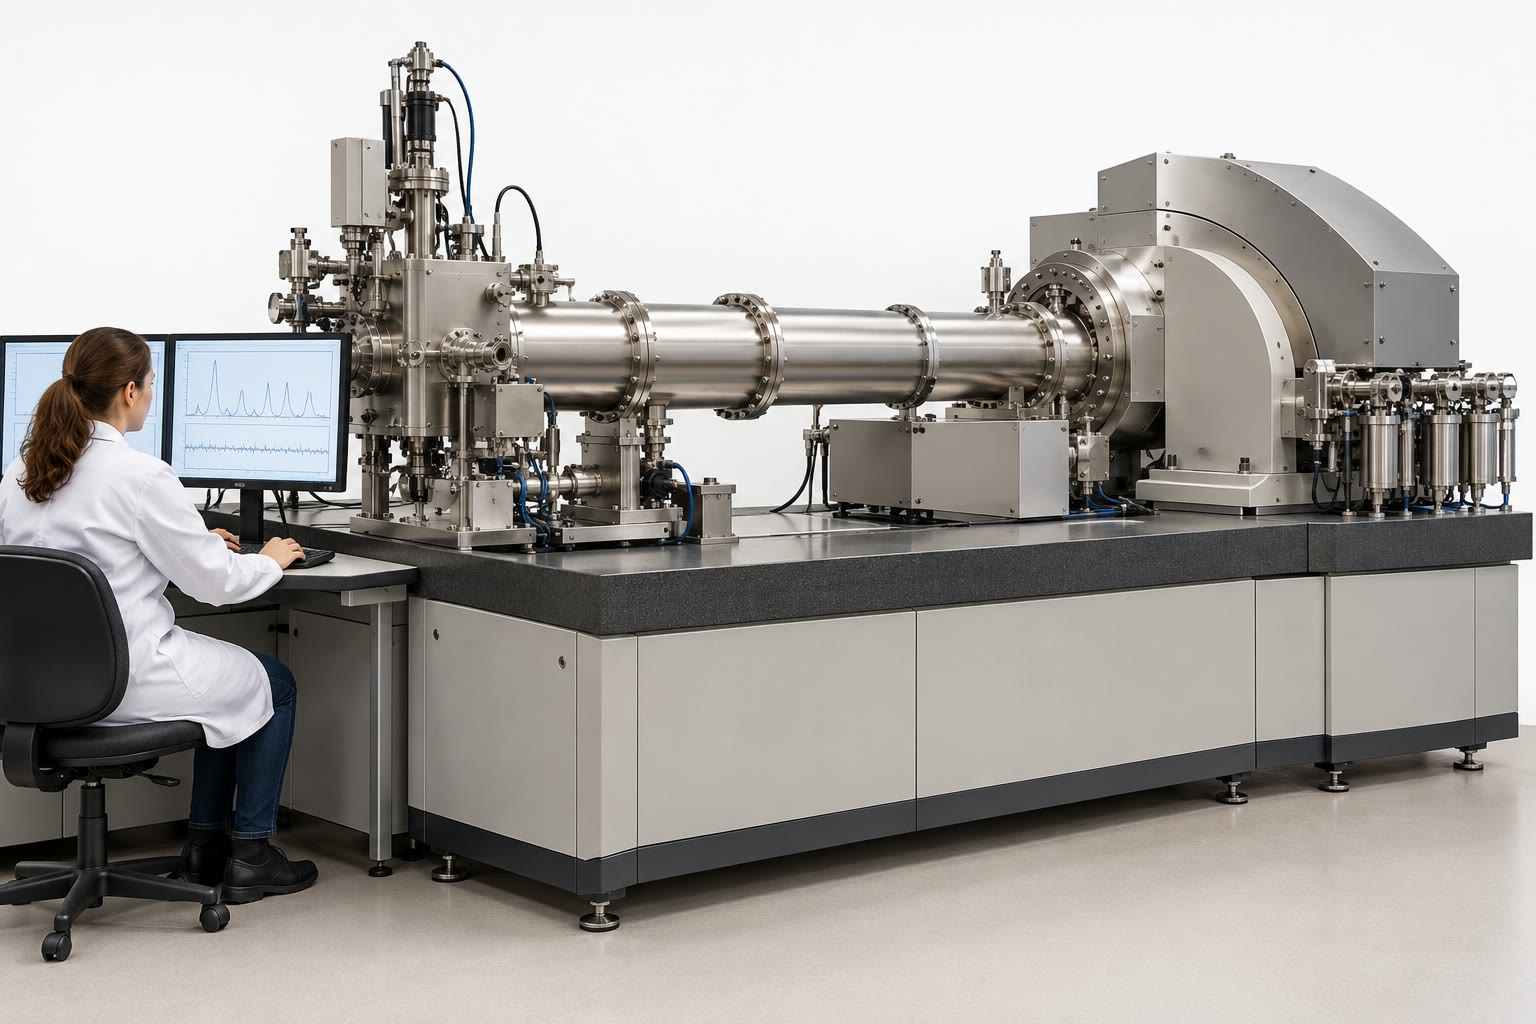
\includegraphics[width=\linewidth]{images/book4/ai/b2-isotope-lab.jpg}
\par\smallskip{\scriptsize A multi-collector mass spectrometer in an isotope
laboratory (AI-generated illustration).}
\end{minipage}
\end{inthelab}
% ledger: white:chur

\section{Exercises}

\begin{exercise}[$\star$]\label{exo:b2:isotope-geochemistry:1}
A basalt from Tristan da Cunha has $^{143}\mathrm{Nd}/^{144}\mathrm{Nd} = 0.51249$ and
one from Mangaia 0.51285. Compute their $\varepsilon_{\mathrm{Nd}}$ and that of the mean
MORB (0.513074). Which sources have had a higher Sm/Nd than \omterm{def:b2:planet-formation-meteorites:chondrule}{chondrites}?
\end{exercise}

\begin{exercise}[$\star$]\label{exo:b2:isotope-geochemistry:2}
The $^{18}\mathrm{O}/^{16}\mathrm{O}$ ratio is \num{2.0052e-3} in \omterm{def:b2:isotope-geochemistry:standards}{VSMOW} and
\num{2.0672e-3} in \omterm{def:b2:isotope-geochemistry:standards}{VPDB}. What is the $\delta^{18}\mathrm{O}$ of \omterm{def:b2:isotope-geochemistry:standards}{VPDB} on the \omterm{def:b2:isotope-geochemistry:standards}{VSMOW}
scale? A calcite has $\delta^{18}\mathrm{O} = -2.0$ per mil (\omterm{def:b2:isotope-geochemistry:standards}{VPDB}); compute its ratio
and its $\delta^{18}\mathrm{O}$ on the \omterm{def:b2:isotope-geochemistry:standards}{VSMOW} scale.
\end{exercise}

\begin{exercise}[$\star$]\label{exo:b2:isotope-geochemistry:3}
Compute the $^{143}\mathrm{Nd}/^{144}\mathrm{Nd}$ of CHUR \qty{1.0}{Ga} ago and
\qty{4.567}{Ga} ago ($\lambda_{147} = \qty{6.524e-12}{\per\year}$,
$^{147}\mathrm{Sm}/^{144}\mathrm{Nd} = 0.1966$, today 0.512638).
\end{exercise}

\begin{exercise}[$\star$]\label{exo:b2:isotope-geochemistry:4}
A snow sample from a mountain station has $\delta^{18}\mathrm{O} = -18.0$ per mil.
What $\delta\mathrm{D}$ does the \omterm{prop:b2:isotope-geochemistry:mwl}{meteoric water line} predict? A lake water has
$\delta^{18}\mathrm{O} = -4.0$ and $\delta\mathrm{D} = -42$ per mil: compute its deuterium
excess $d = \delta\mathrm{D} - 8\delta^{18}\mathrm{O}$, and say whether it lies above or
below the line.
\end{exercise}

\begin{exercise}[$\star\star$]\label{exo:b2:isotope-geochemistry:5}
Evaluate $Q$ of the linear-growth proposition. A granite has Sm \qty{6.0}{ppm}
and Nd \qty{30}{ppm} (CI: 0.145 and \qty{0.457}{ppm}). Compute its
$f_{\mathrm{Sm/Nd}}$, and the change of its $\varepsilon_{\mathrm{Nd}}$ over
\qty{500}{Myr}.
\end{exercise}

\begin{exercise}[$\star\star$]\label{exo:b2:isotope-geochemistry:6}
A crust separated \qty{2.7}{Ga} ago from a mantle with
$\varepsilon_{\mathrm{Nd}} = +3.5$, with $f_{\mathrm{Sm/Nd}} = -0.45$. Estimate its
$\varepsilon_{\mathrm{Nd}}$ today with the linear-growth proposition. The exact
calculation gives $-27.3$; by how much does the approximation differ, and why is it
too high or too low?
\end{exercise}

\begin{exercise}[$\star\star$]\label{exo:b2:isotope-geochemistry:7}
A basaltic magma (Sr \qty{130}{ppm}, $^{87}\mathrm{Sr}/^{86}\mathrm{Sr} = 0.7030$)
assimilates a granite (Sr \qty{320}{ppm}, 0.7200). Compute
$^{87}\mathrm{Sr}/^{86}\mathrm{Sr}$ of mixtures with 5, 10 and 20 per cent granite.
Show that $^{87}\mathrm{Sr}/^{86}\mathrm{Sr}$ is a straight line against $1/\mathrm{Sr}$
and give its slope and intercept.
\end{exercise}

\begin{exercise}[$\star\star$]\label{exo:b2:isotope-geochemistry:8}
With the liquid--vapour fractionation factors 1.0098 ($^{18}$O) and 1.084 (D) at
\qty{20}{\degreeCelsius}, compute the $\delta^{18}\mathrm{O}$ and $\delta\mathrm{D}$ of a
vapour in equilibrium with ocean water (0, 0), and the slope
$\delta\mathrm{D}/\delta^{18}\mathrm{O}$ of the line from the water to the vapour. Repeat
at \qty{0}{\degreeCelsius} (1.0117 and 1.111). Compare with the \omterm{prop:b2:isotope-geochemistry:mwl}{meteoric water line}.
\end{exercise}

\begin{exercise}[$\star\star$]\label{exo:b2:isotope-geochemistry:9}
The continental crust is 0.51 per cent of the mass of the silicate Earth and holds,
on average, \qty{27}{ppm} Nd against \qty{1.25}{ppm} for the silicate Earth. Take
the crust's $\varepsilon_{\mathrm{Nd}}$ as $-15$ and the silicate Earth's as 0. What
share of the neodymium does the crust hold? If the rest of the mantle were uniform,
what would its $\varepsilon_{\mathrm{Nd}}$ be? What share of the neodymium must a
depleted reservoir at $+8.5$ hold if the remainder of the mantle is chondritic?
\end{exercise}

\begin{exercise}[$\star\star\star$]\label{exo:b2:isotope-geochemistry:10}
Show that in the linear-growth proposition the neglected terms are of relative
size about $\lambda t/2$. Over the age of the Earth, how large is this, and how
large an error does it cause in $\varepsilon_{\mathrm{Nd}}$ for $f = -0.45$ over
\qty{2.7}{Ga}?
\end{exercise}

\begin{exercise}[$\star\star\star$]\label{exo:b2:isotope-geochemistry:11}
Two components have Sr/Nd ratios of 13.3 (A) and 5.0 (B). Using the proof of the
\omterm{prop:b2:isotope-geochemistry:mixing}{mixing hyperbola}, find the share $s'$ of strontium from A in a mixture where A
supplies a share $s = 0.5$ of the neodymium. For which value of $s$ do the two
shares differ the most?
\end{exercise}

\begin{exercise}[$\star\star\star$]\label{exo:b2:isotope-geochemistry:12}
A box model gives 2.3 to 2.6 times the present volume of continental crust,
\qty{7.2e9}{km^3}, generated since the Earth formed \qty{4.5}{Ga} ago, and 1.3 to 1.6
times destroyed. Compute the mean rates of generation and destruction in
\unit{km^3} per year. Compare them with the present rates at subduction zones,
\qty{2.7}{km^3} a year added and \qty{3.2}{km^3} a year removed.
\end{exercise}

\section{Problem: Three islands, three mantles}

\begin{problem}[{Weekend problem --- placing the lavas of three islands on the
mantle array, separating a mixture from a third component, and dating the
recycled sediment}]
\label{pb:b2:isotope-geochemistry:1}
Three volcanic islands of an imaginary ocean, Kora, Vel and Asha, erupt basalts
with the isotope ratios below. A geochemist models their sources with two
components: a \omterm{def:b2:isotope-geochemistry:reservoirs}{depleted mantle} like the source of MORB (Sr \qty{10}{ppm}, Nd
\qty{0.75}{ppm}, $^{87}\mathrm{Sr}/^{86}\mathrm{Sr} = 0.70282$,
$^{143}\mathrm{Nd}/^{144}\mathrm{Nd} = 0.51307$) and an old sediment returned to the
mantle by subduction (Sr \qty{200}{ppm}, Nd \qty{40}{ppm}, $0.72000$, $0.51141$;
$^{147}\mathrm{Sm}/^{144}\mathrm{Nd} = 0.110$, $^{87}\mathrm{Rb}/^{86}\mathrm{Sr} = 0.50$).
Kora: $0.70410$, $0.51278$; Vel: $0.70618$, $0.51242$; Asha: $0.70290$, $0.51288$
($^{87}\mathrm{Sr}/^{86}\mathrm{Sr}$, $^{143}\mathrm{Nd}/^{144}\mathrm{Nd}$). CHUR today:
$^{143}\mathrm{Nd}/^{144}\mathrm{Nd} = 0.512638$, $^{147}\mathrm{Sm}/^{144}\mathrm{Nd} =
0.1966$; $\lambda_{147} = \qty{6.524e-12}{\per\year}$, $\lambda_{87} =
\qty{1.3972e-11}{\per\year}$.

\medskip\noindent\textbf{Part I --- Placing the islands.}
\begin{enumerate}
\item Compute $\varepsilon_{\mathrm{Nd}}$ of the two components.
\item Compute $\varepsilon_{\mathrm{Nd}}$ of the three islands.
\item Place the five compositions on a Sr--$\varepsilon_{\mathrm{Nd}}$ diagram. Which
islands lie on the enriched side of CHUR?
\item Asha has nearly the strontium ratio of the \omterm{def:b2:isotope-geochemistry:reservoirs}{depleted mantle} but a much lower
$\varepsilon_{\mathrm{Nd}}$. Where does it plot relative to the mantle array, and which
island group of the chapter does it resemble?
\item Why can the isotope ratios of the lavas be taken as those of their sources,
although the lavas have very different Sm/Nd and Rb/Sr from their sources?
\item A Kora lava with $^{147}\mathrm{Sm}/^{144}\mathrm{Nd} = 0.12$ is \qty{1}{Myr} old.
By how much has its $^{143}\mathrm{Nd}/^{144}\mathrm{Nd}$ grown since eruption, in
epsilon units? Does this matter?
\end{enumerate}

\noindent\textbf{Part II --- Mixing the two components.}
\begin{enumerate}[resume]
\item Write the Nd concentration and the $^{143}\mathrm{Nd}/^{144}\mathrm{Nd}$ of a
mixture with a mass fraction $f$ of sediment.
\item Compute $\varepsilon_{\mathrm{Nd}}$ of mixtures with $f = 0.5$, 1, 2 and 5 per
cent.
\item Compute $^{87}\mathrm{Sr}/^{86}\mathrm{Sr}$ of the same mixtures.
\item Show that the $^{87}\mathrm{Sr}/^{86}\mathrm{Sr}$ of the mixtures is a straight
line against $1/\mathrm{Sr}$, and give its slope.
\item Compute $K = (\mathrm{Sr}/\mathrm{Nd})_{\text{mantle}}/(\mathrm{Sr}/\mathrm{Nd})_{\text{sediment}}$.
Which ratio, Sr or Nd, moves towards the sediment faster as $f$ grows?
\item By how many times is the sediment richer than the mantle in Nd, and in Sr?
Explain with these numbers why one per cent of sediment shifts
$\varepsilon_{\mathrm{Nd}}$ by about 11 units.
\item What share of the neodymium of a mixture with $f = 1$ per cent comes from the
sediment?
\end{enumerate}

\noindent\textbf{Part III --- How much sediment?}
\begin{enumerate}[resume]
\item Solve the Nd mixing equation for $f$, given the ratio $R$ of the mixture.
\item Compute $f$ for Kora from its neodymium.
\item Compute $f$ for Kora from its strontium. Do the two agree?
\item Compute $f$ for Vel from its neodymium and from its strontium.
\item Compute $f$ for Asha from its neodymium, and the strontium ratio this $f$
predicts. Compare with the measured value: what do you conclude about Asha's
source?
\item Suggest a third component for Asha, from the chapter, and the
parent--daughter ratios it must have had.
\end{enumerate}

\noindent\textbf{Part IV --- The age of the sediment.}
\begin{enumerate}[resume]
\item The sediment was subducted \qty{2.0}{Ga} ago and has been closed since.
Compute its $^{143}\mathrm{Nd}/^{144}\mathrm{Nd}$, that of CHUR and its
$\varepsilon_{\mathrm{Nd}}$ at that time.
\item Redo the calculation with the linear-growth proposition.
\item Compute the $^{87}\mathrm{Sr}/^{86}\mathrm{Sr}$ of the sediment \qty{2.0}{Ga} ago.
\item \qty{2.0}{Ga} ago, the crust of the $\varepsilon_{\mathrm{Nd}}$ figure had
$\varepsilon_{\mathrm{Nd}} \approx -4.7$. Is the sediment's value at subduction consistent
with an origin by erosion of such young continental crust?
\item State the mass fraction of recycled sediment in the source of the most
enriched island, the key number of this problem.
\end{enumerate}
\end{problem}
% ledger: white:chur, villa20:sm147, villa22:rb87, gale13:isotopes
